\definecolor{wsdred}{HTML}{8E1728}



\tikzset{every picture/.style={line width=0.75pt}} %set default line width to 0.75pt        

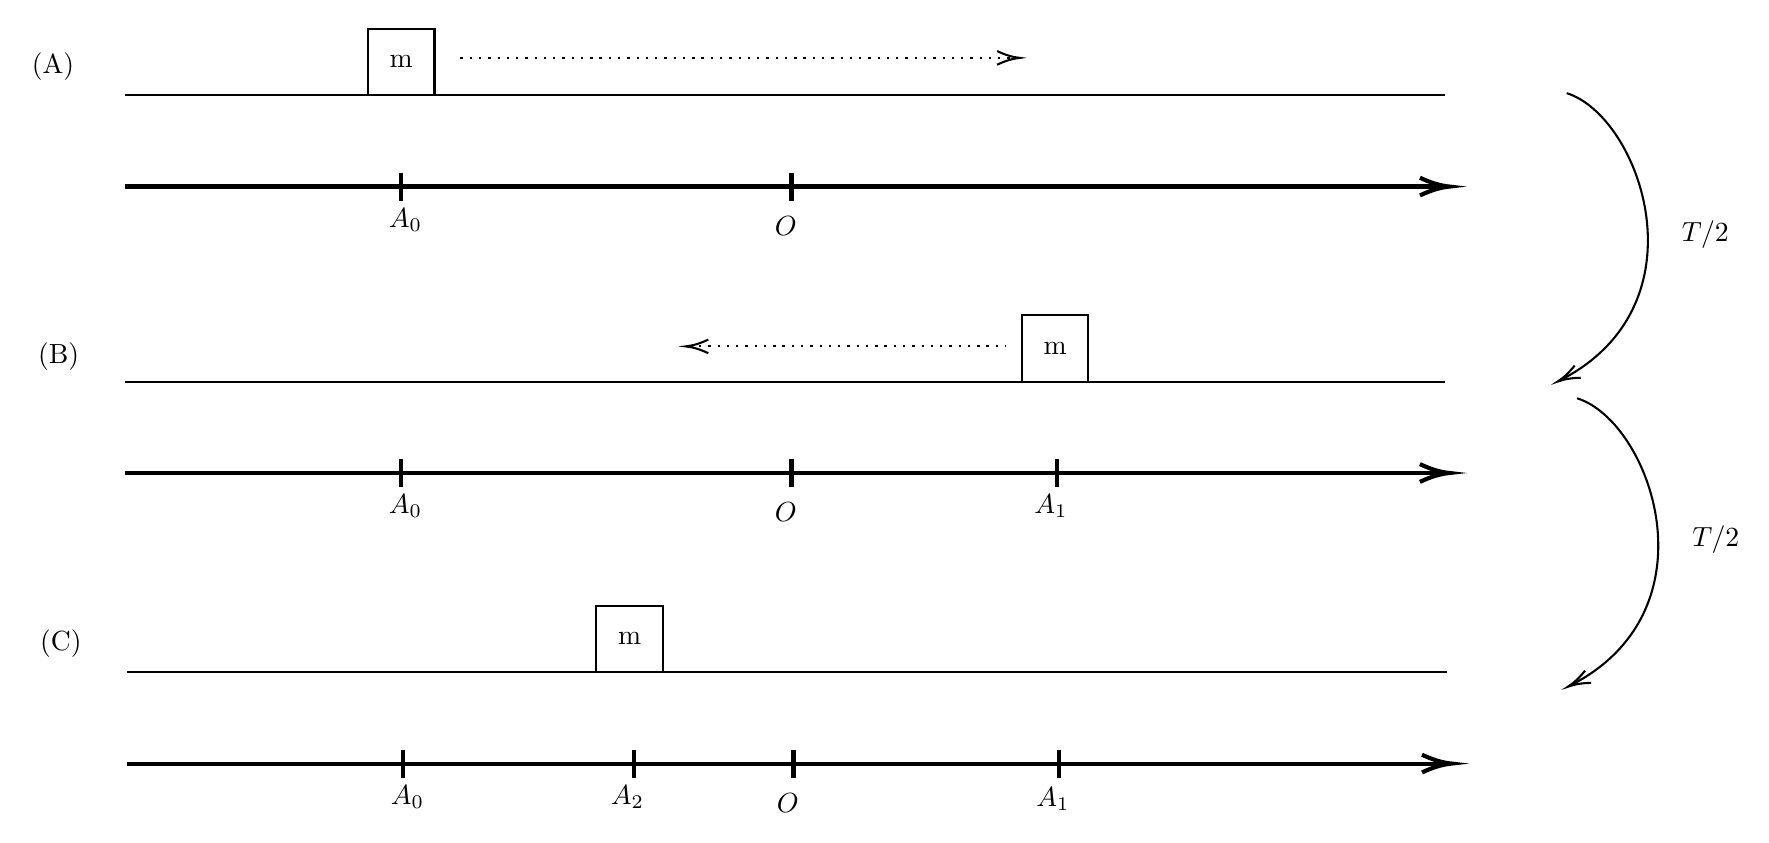
\begin{tikzpicture}[x=0.75pt,y=0.75pt,yscale=-1,xscale=1]
%uncomment if require: \path (0,15225); %set diagram left start at 0, and has height of 15225

%Straight Lines [id:da8440235981456923] 
\draw [color={rgb, 255:red, 0; green, 0; blue, 0 }  ,draw opacity=1 ]   (748.5,4556) -- (112.5,4556) ;
%Shape: Square [id:dp7730743948956422] 
\draw  [color={rgb, 255:red, 0; green, 0; blue, 0 }  ,draw opacity=1 ] (229.5,4524) -- (261.5,4524) -- (261.5,4556) -- (229.5,4556) -- cycle ;
%Straight Lines [id:da5849410238032737] 
\draw [color={rgb, 255:red, 0; green, 0; blue, 0 }  ,draw opacity=1 ][line width=1.5]    (433.5,4600) -- (747.5,4600) ;
\draw [shift={(750.5,4600)}, rotate = 180] [color={rgb, 255:red, 0; green, 0; blue, 0 }  ,draw opacity=1 ][line width=1.5]    (14.21,-4.28) .. controls (9.04,-1.82) and (4.3,-0.39) .. (0,0) .. controls (4.3,0.39) and (9.04,1.82) .. (14.21,4.28)   ;
%Straight Lines [id:da501337374602] 
\draw [color={rgb, 255:red, 0; green, 0; blue, 0 }  ,draw opacity=1 ][line width=1.5]    (245.5,4600) -- (433.5,4600) ;
\draw [shift={(433.5,4600)}, rotate = 180] [color={rgb, 255:red, 0; green, 0; blue, 0 }  ,draw opacity=1 ][line width=1.5]    (0,6.71) -- (0,-6.71)   ;
%Straight Lines [id:da8338549647082345] 
\draw [color={rgb, 255:red, 0; green, 0; blue, 0 }  ,draw opacity=1 ][line width=1.5]    (112.5,4600) -- (245.5,4600) ;
\draw [shift={(245.5,4600)}, rotate = 180] [color={rgb, 255:red, 0; green, 0; blue, 0 }  ,draw opacity=1 ][line width=1.5]    (0,6.71) -- (0,-6.71)   ;
%Straight Lines [id:da5472639759035778] 
\draw [color={rgb, 255:red, 0; green, 0; blue, 0 }  ,draw opacity=1 ]   (748.5,4694) -- (112.5,4694) ;
%Shape: Square [id:dp11345606497116645] 
\draw  [color={rgb, 255:red, 0; green, 0; blue, 0 }  ,draw opacity=1 ] (544.5,4662) -- (576.5,4662) -- (576.5,4694) -- (544.5,4694) -- cycle ;
%Straight Lines [id:da28185616117474566] 
\draw [color={rgb, 255:red, 0; green, 0; blue, 0 }  ,draw opacity=1 ][line width=1.5]    (433.5,4738) -- (747.5,4738) ;
\draw [shift={(750.5,4738)}, rotate = 180] [color={rgb, 255:red, 0; green, 0; blue, 0 }  ,draw opacity=1 ][line width=1.5]    (14.21,-4.28) .. controls (9.04,-1.82) and (4.3,-0.39) .. (0,0) .. controls (4.3,0.39) and (9.04,1.82) .. (14.21,4.28)   ;
%Straight Lines [id:da614812825007393] 
\draw [color={rgb, 255:red, 0; green, 0; blue, 0 }  ,draw opacity=1 ][line width=1.5]    (245.5,4738) -- (433.5,4738) ;
\draw [shift={(433.5,4738)}, rotate = 180] [color={rgb, 255:red, 0; green, 0; blue, 0 }  ,draw opacity=1 ][line width=1.5]    (0,6.71) -- (0,-6.71)   ;
%Straight Lines [id:da3151466941990222] 
\draw [color={rgb, 255:red, 0; green, 0; blue, 0 }  ,draw opacity=1 ][line width=1.5]    (112.5,4738) -- (245.5,4738) ;
\draw [shift={(245.5,4738)}, rotate = 180] [color={rgb, 255:red, 0; green, 0; blue, 0 }  ,draw opacity=1 ][line width=1.5]    (0,6.71) -- (0,-6.71)   ;
%Straight Lines [id:da16801387670839896] 
\draw [color={rgb, 255:red, 0; green, 0; blue, 0 }  ,draw opacity=1 ][line width=1.5]    (433.5,4738) -- (561.5,4738) ;
\draw [shift={(561.5,4738)}, rotate = 180] [color={rgb, 255:red, 0; green, 0; blue, 0 }  ,draw opacity=1 ][line width=1.5]    (0,6.71) -- (0,-6.71)   ;
%Straight Lines [id:da7824565205771314] 
\draw [color={rgb, 255:red, 0; green, 0; blue, 0 }  ,draw opacity=1 ]   (749.5,4834) -- (113.5,4834) ;
%Shape: Square [id:dp10726696816762793] 
\draw  [color={rgb, 255:red, 0; green, 0; blue, 0 }  ,draw opacity=1 ] (339.5,4802) -- (371.5,4802) -- (371.5,4834) -- (339.5,4834) -- cycle ;
%Straight Lines [id:da5556513504225804] 
\draw [color={rgb, 255:red, 0; green, 0; blue, 0 }  ,draw opacity=1 ][line width=1.5]    (434.5,4878) -- (748.5,4878) ;
\draw [shift={(751.5,4878)}, rotate = 180] [color={rgb, 255:red, 0; green, 0; blue, 0 }  ,draw opacity=1 ][line width=1.5]    (14.21,-4.28) .. controls (9.04,-1.82) and (4.3,-0.39) .. (0,0) .. controls (4.3,0.39) and (9.04,1.82) .. (14.21,4.28)   ;
%Straight Lines [id:da35868213260288484] 
\draw [color={rgb, 255:red, 0; green, 0; blue, 0 }  ,draw opacity=1 ][line width=1.5]    (246.5,4878) -- (434.5,4878) ;
\draw [shift={(434.5,4878)}, rotate = 180] [color={rgb, 255:red, 0; green, 0; blue, 0 }  ,draw opacity=1 ][line width=1.5]    (0,6.71) -- (0,-6.71)   ;
%Straight Lines [id:da9226047069569581] 
\draw [color={rgb, 255:red, 0; green, 0; blue, 0 }  ,draw opacity=1 ][line width=1.5]    (113.5,4878) -- (246.5,4878) ;
\draw [shift={(246.5,4878)}, rotate = 180] [color={rgb, 255:red, 0; green, 0; blue, 0 }  ,draw opacity=1 ][line width=1.5]    (0,6.71) -- (0,-6.71)   ;
%Straight Lines [id:da39824710137073915] 
\draw [color={rgb, 255:red, 0; green, 0; blue, 0 }  ,draw opacity=1 ][line width=1.5]    (434.5,4878) -- (562.5,4878) ;
\draw [shift={(562.5,4878)}, rotate = 180] [color={rgb, 255:red, 0; green, 0; blue, 0 }  ,draw opacity=1 ][line width=1.5]    (0,6.71) -- (0,-6.71)   ;
%Straight Lines [id:da5711245809745336] 
\draw [color={rgb, 255:red, 0; green, 0; blue, 0 }  ,draw opacity=1 ][line width=1.5]    (357.5,4878) -- (434.5,4878) ;
\draw [shift={(357.5,4878)}, rotate = 180] [color={rgb, 255:red, 0; green, 0; blue, 0 }  ,draw opacity=1 ][line width=1.5]    (0,6.71) -- (0,-6.71)   ;
%Straight Lines [id:da2785554999977735] 
\draw [color={rgb, 255:red, 0; green, 0; blue, 0 }  ,draw opacity=1 ] [dash pattern={on 0.84pt off 2.51pt}]  (274,4538) -- (541.5,4538) ;
\draw [shift={(543.5,4538)}, rotate = 180] [color={rgb, 255:red, 0; green, 0; blue, 0 }  ,draw opacity=1 ][line width=0.75]    (10.93,-3.29) .. controls (6.95,-1.4) and (3.31,-0.3) .. (0,0) .. controls (3.31,0.3) and (6.95,1.4) .. (10.93,3.29)   ;
%Straight Lines [id:da5363770674501016] 
\draw [color={rgb, 255:red, 0; green, 0; blue, 0 }  ,draw opacity=1 ] [dash pattern={on 0.84pt off 2.51pt}]  (384.5,4677) -- (536.5,4677) ;
\draw [shift={(382.5,4677)}, rotate = 0] [color={rgb, 255:red, 0; green, 0; blue, 0 }  ,draw opacity=1 ][line width=0.75]    (10.93,-3.29) .. controls (6.95,-1.4) and (3.31,-0.3) .. (0,0) .. controls (3.31,0.3) and (6.95,1.4) .. (10.93,3.29)   ;
%Curve Lines [id:da8774718138615303] 
\draw [color={rgb, 255:red, 0; green, 0; blue, 0 }  ,draw opacity=1 ]   (807,4555) .. controls (842.32,4565.95) and (875.17,4657.08) .. (803.59,4693.46) ;
\draw [shift={(802.5,4694)}, rotate = 333.75] [color={rgb, 255:red, 0; green, 0; blue, 0 }  ,draw opacity=1 ][line width=0.75]    (10.93,-3.29) .. controls (6.95,-1.4) and (3.31,-0.3) .. (0,0) .. controls (3.31,0.3) and (6.95,1.4) .. (10.93,3.29)   ;
%Curve Lines [id:da6809827298064757] 
\draw [color={rgb, 255:red, 0; green, 0; blue, 0 }  ,draw opacity=1 ]   (812,4702) .. controls (847.32,4712.95) and (880.17,4804.08) .. (808.59,4840.46) ;
\draw [shift={(807.5,4841)}, rotate = 333.75] [color={rgb, 255:red, 0; green, 0; blue, 0 }  ,draw opacity=1 ][line width=0.75]    (10.93,-3.29) .. controls (6.95,-1.4) and (3.31,-0.3) .. (0,0) .. controls (3.31,0.3) and (6.95,1.4) .. (10.93,3.29)   ;

% Text Node
\draw (245.5,4540) node   [align=left] {\textcolor{black}{m}};
% Text Node
\draw (424,4613) node [anchor=north west][inner sep=0.75pt]    {\textcolor{black}{$O$}};
% Text Node
\draw (238,4609) node [anchor=north west][inner sep=0.75pt]    {\textcolor{black}{$A_{0}$}};
% Text Node
\draw (560.5,4678) node   [align=left] {\textcolor{black}{m}};
% Text Node
\draw (424,4751) node [anchor=north west][inner sep=0.75pt]    {\textcolor{black}{$O$}};
% Text Node
\draw (238,4747) node [anchor=north west][inner sep=0.75pt]    {\textcolor{black}{$A_{0}$}};
% Text Node
\draw (549,4747) node [anchor=north west][inner sep=0.75pt]    {\textcolor{black}{$A_{1}$}};
% Text Node
\draw (355.5,4818) node   [align=left] {\textcolor{black}{m}};
% Text Node
\draw (425,4891) node [anchor=north west][inner sep=0.75pt]    {\textcolor{black}{$O$}};
% Text Node
\draw (239,4887) node [anchor=north west][inner sep=0.75pt]    {\textcolor{black}{$A_{0}$}};
% Text Node
\draw (550,4888) node [anchor=north west][inner sep=0.75pt]    {\textcolor{black}{$A_{1}$}};
% Text Node
\draw (345,4887) node [anchor=north west][inner sep=0.75pt]    {\textcolor{black}{$A_{2}$}};
% Text Node
\draw (861,4615) node [anchor=north west][inner sep=0.75pt]    {\textcolor{black}{$T/2$}};
% Text Node
\draw (866,4762) node [anchor=north west][inner sep=0.75pt]    {\textcolor{black}{$T/2$}};
% Text Node
\draw (66,4534) node [anchor=north west][inner sep=0.75pt]   [align=left] {(A)};
% Text Node
\draw (69,4674) node [anchor=north west][inner sep=0.75pt]   [align=left] {(B)};
% Text Node
\draw (70,4812) node [anchor=north west][inner sep=0.75pt]   [align=left] {(C)};


\end{tikzpicture}